Chaque service que nous mettons en place nécéssite implicitement d'être hébergé quelque part. N'ayant pas les moyens de nous offrir un VPS pour le déploiement de l'intégralité des services sur lesquels nous avons travaillé, nous avons pris l'opportunité de déployer ces derniers sur un serveur mis à disposition pour le projet à l'école.

Ce serveur est une machine HP de type rack 1U qui fait tourner le système d'exploitation ESXi\footnote{OS de gestion de machines virtuelles de VMware}. Grâce à cela, nous pouvons lancer des machines virtuelles sur lesquelles tourneront nos différents systèmes d'exploitation.

Bien évidemment, dans un scénario plus réaliste, nous n'aurions pas seulement un serveur, mais plusieurs. Les ressources de l'école nous limite à n'utiliser qu'un serveur physique. Nous considèrerons alors que chaque système d'exploitation tournant sur ESXi soit en fait un serveur physique qui va, plus tard, faire partie d'un "cluster". Je vais revenir sur ce terme là un peu plus tard.

\section{Virtualisation des services}

\begin{figure}[H]
    \centering
    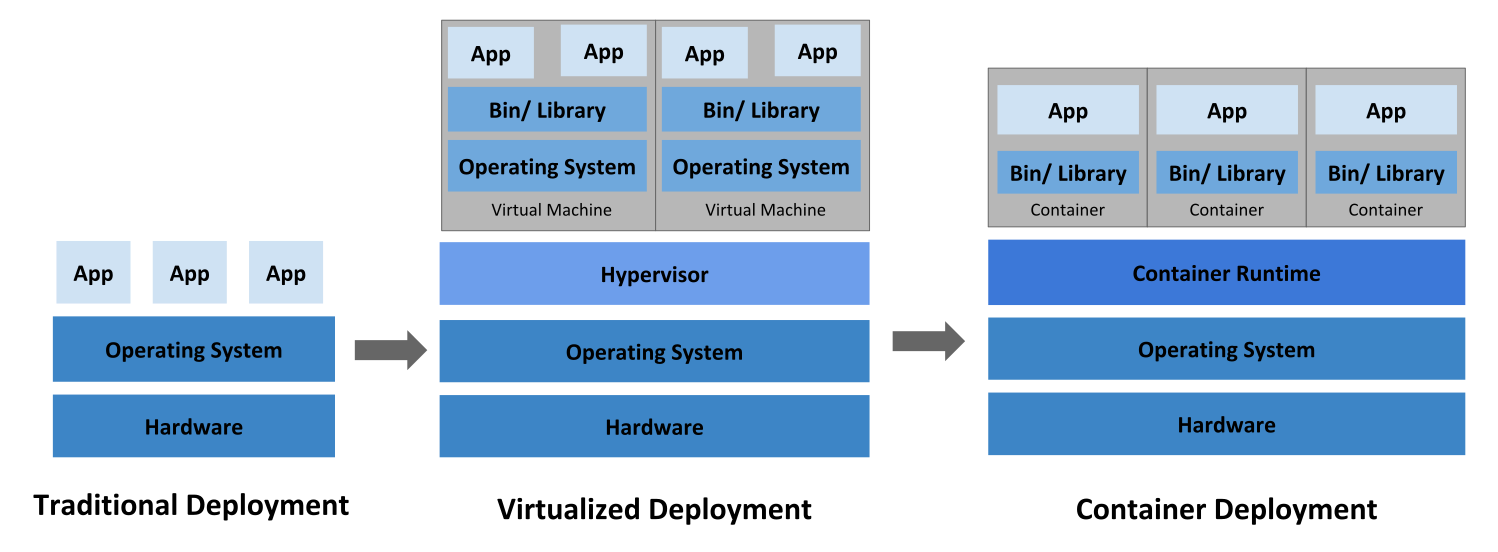
\includegraphics[width=\textwidth]{./img/container_evolution.png}
    \caption{Évolution du déploiement d'applications \cite{shavidissa2019}}
    \label{fig:container_evolution}
\end{figure}

Traditionnellement, lorsqu'une application devait être déployée et rendue utile au grand public, elle était simplement exécutée sur le système d'exploitation de la machine physique hôte. Ce "déploiement traditionnel", qui, à la surface, semblait simple, posait en fait, au long terme, bien des problèmes. On peut citer des problèmes de sécurité car l'application cohabiterai avec d'autres applications ou bien des problèmes de scalabilité, où les applications sont limités au niveau des ressources qu'offre le hardware de la machine, mais aussi des problèmes où l'application dépendrait de l'intégrité du système dans lequel elle est installée.

Pour palier à tout ça, une des solutions est de travailler avec des machines virtuelles. Un hyperviseur va pouvoir orchestrer différents systèmes d'exploitation dans lesquels résideront les services que nous souhaitons déployer. Ainsi, chaque service sera isolé des autres. De plus, il est possible de mettre en place un système qui, en cas de défaut d'une instance d'un service ou en cas de demande saturée du service, il est possible de lancer, à la volée, une machine virtuelle qui ferait tourner ce service. Rendant ainsi possible un load balancing des requêtes envers ce service. Un des seuls soucis avec tout ça, c'est que l'utilisation des machines virtuelles présente un overhead plutôt conséquent.

La solution que nous avons opté découle des deux solutions ci-dessus. Elle améliore le service en le redant:

\begin{itemize}
    \item plus isolé
    \item plus facilement instanciable
    \item moins coûteux en terme d'overhead
\end{itemize}

Le principe est d'avoir plusieures machines présentant chacune leur propre système d'exploitation (ici, Linux\footnote{ou plus précisément, Ubuntu 23.04}). Dans ces systèmes d'exploitation tourneront des moteurs de containerization, comme Docker.

\subsection{Docker}

Comme dit précédemment, La technologie de containerization que nous allons utiliser s'appelle Docker. Elle permet de "construire" notre propre container avec le service que nous souhaitons déployer. Il restera alors à dire à Docker de déployer un service untel et le service se déploiera\dots N'est-ce pas ?

Certains d'entre vous me diront "Mais Flo, qu'en est-il de l'orchestration des différents services, tu sais, l'avantage que nous présentais le deuxième point ?". Malheureusement, jeune padawan, Docker ne nous permets pas ça. Il permet d'isoler un environnemnt mais sur qu'une seule machine. Travailler en harmonie avec d'autres moteurs docker reste impossible\dots ou du moins sans notre dernière solution.

\section{Kubernetes}

Kubernetes fait partie de la famille des orchestrateur de containers. C'est une couche au dessus qui va s'occuper de lancer  des pods\footnote{l'unité la plus petite de kubernetes. Elle comprend un ou plusieurs containeurs qui travaillent ensemble} dans un cluster\footnote{un groupe} de nodes\footnote{les serveurs sur lesquels vont tourner les containers}.

Notre but étant que, à la place d'avoir une structure verticale de plusieures machines qui s'occuperont de nos services, nous avons opté sur une structure horizontale. Le principal est que, depuis un entrypoint singulier (ici, l'ingress), on peut accéder plusieurs différents services.

\subsection{Administration du cluster}

L'administration du cluster est une épreuve assez fastidieuse. Je vais décrire ici les différents aspects de la gestion de cluster:

\paragraph{Initialisation du cluster:} pour cette étape, il faut lancer la commande kubeadm init sur le serveur qui agira comme master. Il faut ensuite spécifier plusieurs paramètres:
\begin{itemize}
    \item \mintinline{shell}|--apiserver-advertise-address| étant donné que je travaille sur un serveur avec plusieurs interfaces réseaux (une interface pour la connexion entre les nodes et une interface qui fait connexion temporaire internet), j'ai dû préciser l'adresse IP sur laquelle on écoute les appels vers l'API Kubernetes\footnote{l'API est le moyen principal pour que les nodes communiquent entre-eux. Ils communiques par HTTP et l'API se situe sur le master-node}. En l'occurence, j'y ai mis l'IP 172.16.100.18/29.
    \item \mintinline{shell}|--cri-socket| étant donné que Kubernetes est totalement indépendant de gestionnaire de containers, il faut pouvoir spécifier un CRI, c'est-à-dire un Container Runtime Interface.\footnote{vous l'aurez compris, nous avons choisi Docker pour remplir ce rôle}
    \item \mintinline{shell}|--pod-network-cidr| nous ne l'avons pas utilisé, mais il est important de spécifier que ce dernier permet de spécifier un network virtuel sur lesquels vont communiquer les pods. Il est indifférent des networks physiques que nous avons mis en place.
\end{itemize}
L'initialisation du cluster finie, il faut ensuite pouvoir joindre les worker nodes avec la commande kubeadm join, prenant en paramètre l'adresse IP du master node.

\paragraph{Container Network Interface plugin:} un inconvéniant et un avantage de kubernetes est l'utilisation obligatoire d'un plugin d'interface réseau. Aux premiers abords, j'ai trouvé ça perturbant, surtout sur "comment choisir le bon plugin ?". Ayant creusé un peu, j'ai finalement pu prendre le plugin Flannel, qui est plus ou moins populaire. Cependant, il est intéressant de noter que certains plugins peuvent prendre en compte le protocol BGP ou peut permettre bien d'autres choses. Je ne vais pas rentrer dans les détails cependant. Le déploiement du plugin se fait sur le node master et se répliquera dans les nodes workers automatiquement.

\paragraph{Container Storage Interface:} le dernier obstacle qui me barrait la route au bon fonctionnement d'un déploiement d'un pod sur le cluster était la mise en place d'un système de stockage. Le principe du système de stockage dans Kubernetes est de créer ce qu'on appelle des "Persistant Volume". Après la création desdits storages, un pod va demander une certaine taille de stockage avec un "Persistant Volume Claim". Nous avons choisi la façon la plus basique de stocker des données, c'est à dire sous un dossier dans une VM. Mais il est cependant possible de le faire avec du iSCSI, avec vSphere, GKE, AWS etc.

\paragraph{Serveur de Certificat Authoritaire:} afin de permettre une connexion sécurisée entre un client et les service que l'on met en place, il nous faut un certificat authoritaire qui va s'occuper des différents services. Mieux encore, nous avons opté sur un serveur qui accepte le protocol ACME, ainsi, il sera possible d'automatiser le renouvellement de certificats grâce au service suivant.

\paragraph{Ingress Nginx:} ceci n'est pas réellement obligatoire au fonctionnement du déploiement, mais j'ai préféré l'utiliser. C'est un plugin qui va faire office de reverse proxy. C'est-à-dire qu'en fonction de l'addresse DNS rensegnée dans la requête, le reverse proxy va rediriger la requête vers le bon service. 

Pour exposer l'ensemble des services sur l'externe, j'ai choisi d'utiliser un NodePort. Avec un NodePort, on va assigner un service (ici, le ingress nginx) sur un port spécifique. Ainsi, le service nginx va être constamment accessible via n'importe quele addresse IP d'un node et le port spécifié dans la configuration d'un NodePort.

\begin{figure}[H]
    \centering
    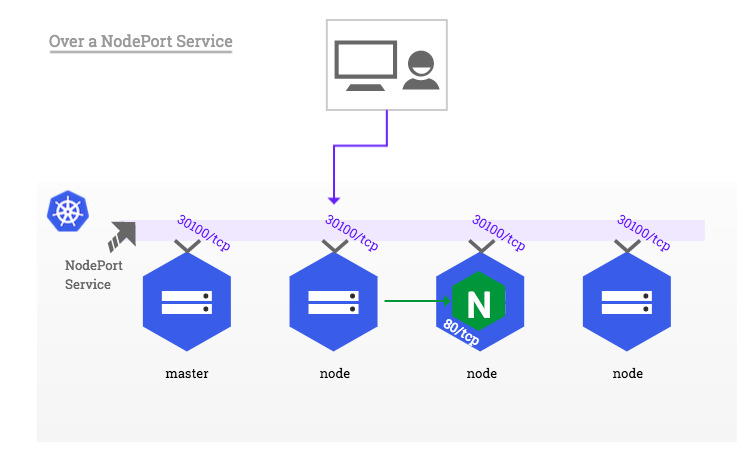
\includegraphics[width=\textwidth]{./img/nodeport.jpg}
    \caption{Représentation graphique d'un NodePort}
    \label{fig:node_port}
\end{figure}

\subsection{Mise en place du déploiement}

Chaque service que nous avons développé/travaillé dessus va se voir être hébergé sur le cluster. Nous avons créé certains containers grâce à des Dockerfiles, tandis que certains autres services fonctionne via docker compose. Heureusement pour nous, Kubernetes a un outils qui s'appelle "Konvert" et permet de convertir un docker-compose en pods kubernetes.

\section{Outil de build et système de contrôle de version}

\subsection{Git \& le contrôle de version}

Git, outil bien connu de tout développeur, a été la principale façon pour nous de partager notre code. Nous avons mis en commun notre code sur la plateforme GitHub, sous une organisation créée pour l'occasion. Chacun allait pouvoir créer un repository pour chaque projet qu'il comptait ajouter à la solution finale. De plus, github nous permet de gérer un repository d'images Docker et de librairies Maven qui nous permettra, in fine, de les téléverser dessus.

\subsection{Gradle, l'outil de build logiciel}

Comme la majorité des personnes de notre groupe souhaitait travailler avec le JVM, j'ai voulu mettre en place un moyen pour eux de simplement entrer le plugin correspondant à leur type de projet dans leur gradle, et ainsi ils n'avaient qu'à coder. Ils ne devaient pas se soucier de "comment déployer l'application".

Il y avait trois types d'applications:

\begin{itemize}
    \item L'application finale: c'est-à-dire une application lancée par un utilisateur final. Cette dernière peut-être l'application mobile ou bien l'application desktop de lecture de carte d'identité. Ces applications ne nécessitaient pas réellement de déploiement à proprement parlé.
    \item L'application serveur: ce type d'application va être héberger sur un serveur. Dans notre cas, ça sera dans le cluster Kubernetes mis en place précédemment. Le principal est alors de placer tout ça dans un container docker. Jib, un plugin gradle spécialiser dans la containerization de services du JVM, a été le plugin de choix pour créer un docker et pour pouvoir le téléverser sur GitHub Packages.
    \item L'application librairie: \footnote{résultante d'un abus de language, une application n'est pas forcément une librairie} ces dernières sont similaire aux containers Docker, à la différence qu'elle seront hébergées sur un serveur Maven, aussi offert par Github.
\end{itemize}
